\documentclass[12pt]{article}
\usepackage{fontspec}
\usepackage{xeCJK}
\setCJKmainfont[AutoFakeBold=2]{SimSun}
%\setCJKsansfont{SimHei}
\usepackage{amsmath, amssymb, amsthm}
\usepackage{geometry}
\usepackage{tikz}
\usepackage{fancyhdr}
%\setlength{\headheight}{15pt}
\usetikzlibrary{calc, intersections} % ABX 用於某些符號，若無可刪除
\usepackage{enumitem}
\usepackage{tkz-euclide}
\usepackage[most]{tcolorbox}
\newtcolorbox{mybox}[3][證明]{
  empty,
  breakable,                % 支援跨頁
  sharp corners,
  left=#2+#3,               % 為左側標籤預留空間 (縮進)
  right=0pt, top=0pt, bottom=0pt,
  colback=white,
  overlay unbroken and first={ % 在第一頁/未斷頁時繪製標籤
    \node[
      anchor=north west,
      draw, 
      inner sep=0pt,
      minimum width=#2,
      minimum height=1.6em, % 你可以根據字體調整高度
      font=\bfseries\boldmath
    ] at (frame.north west) {#1};
  }
}
\setlength{\headheight}{15pt} % 避免頁首高度警告

\geometry{left=1.5cm, right=1.5cm, top=2cm, bottom=2cm}

% 設定頁首頁尾
\pagestyle{fancy}
\fancyhf{}
\renewcommand{\headrulewidth}{2pt}
\lhead{廖汶鋒}
\chead{幾何能力測評題}
\rhead{澳門培道中學}
\fancyfoot[C]{\thepage} % Centered footer
\fancyfoot[L]{2026年2月7日} % Left footer

%\title{幾何能力測評題}
%\author{廖汶鋒}
%\date{2026年1月24日$\sim$\ 2026年2月1日}
\linespread{1.3}

% 設定段落首行縮進（兩個中文字）
\setlength{\parindent}{2em}

\begin{document}

\thispagestyle{fancy}  % 讓首頁也顯示頁首
%\maketitle
\begin{center}
  \textbf{\Large{能力測評題答案}}
\end{center}
請不要利用任何AI工具或互聯網資源解答以下問題，並在解答過程中完成尺規作圖。\\[1em]

\begin{mybox}[問題1]{4em}{1em}
    設$\Omega$與$\Gamma$分別是以後$M,N$為圓心的圓，且圓$\Omega$的半徑小於圓$\Gamma$的半徑。
    設$\Omega$與$\Gamma$交於相異兩點$A,B$。直線$MN$與圓$\Omega$交於點$C$、與圓$\Gamma$交於點$D$，
    且$C,M,N,D$四點依此順序落在該直線上。直線$AP$與圓$\Omega$交於點$E\neq A$、與圓$\Gamma$再交於點$F\neq A$。
    令點$H$為$\triangle{PMN}$的垂心。\\[0.5em]
    求證：通過$H$且平行於$AP$的直線$l$，與$\triangle{BEF}$的外接圓相切。
    
    \begin{center}
      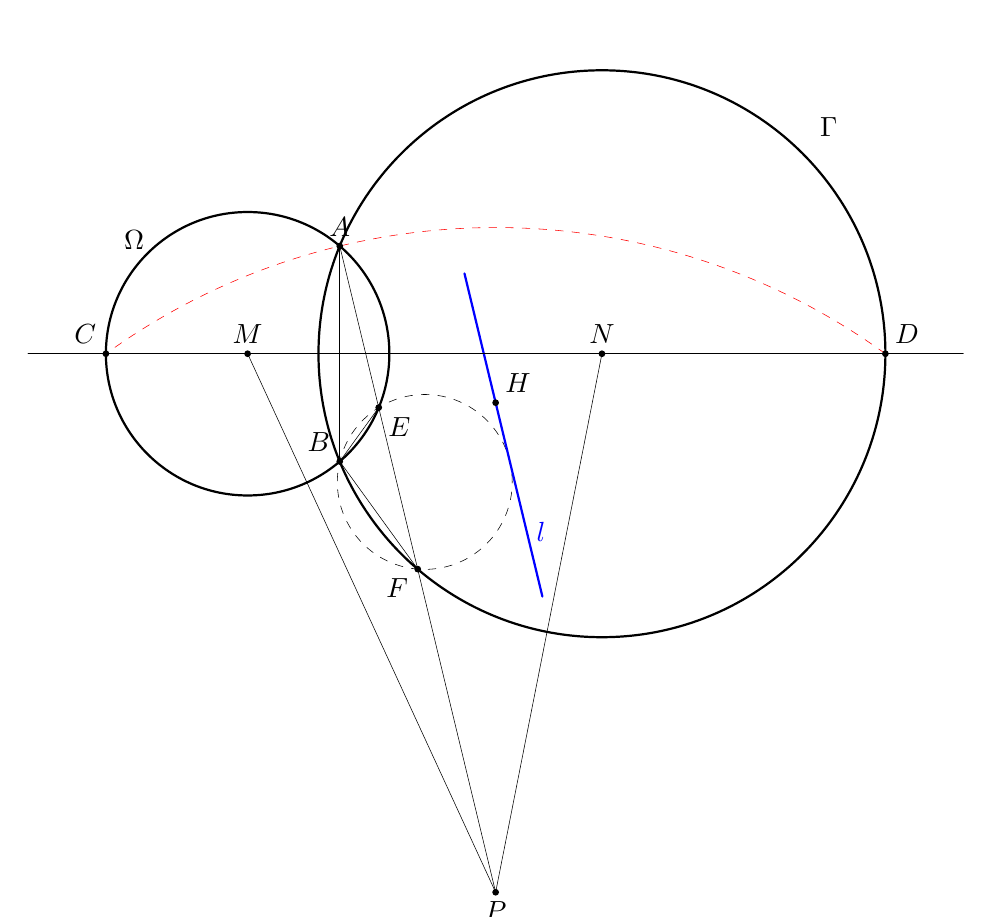
\begin{tikzpicture}[scale=0.9]
          % --- 1. 定義圓心 M, N 與半徑 ---
          \tkzDefPoint(-2,0){M}
          \tkzDefPoint(3,0){N}
          \def\rO{2}
          \def\rG{4}
          
          % --- 2. 定義直線 MN 上的 C, D (確保 C, M, N, D 順序) ---
          \tkzDefPoint(-2-\rO,0){C}
          \tkzDefPoint(3+\rG,0){D}
          
          % --- 3. 繪製兩圓 Omega, Gamma ---
          \tkzDrawCircle[thick,black](M,C)
          \tkzDrawCircle[thick,black](N,D)
          
          % --- 4. 求兩圓交點 A, B ---
          \tkzInterCC(M,C)(N,D) \tkzGetPoints{A}{B}
          
          % --- 5. 定義 P 為三角形 ACD 的外心 ---
          \tkzCircumCenter(A,C,D) \tkzGetPoint{P}
          %\tkzDrawCircle[dashed, cyan](P,A) % 繪製 ACD 的外接圓供參考
          \tkzDrawArc[color=red, dashed](P,D)(C)
          % --- 6. 構造割線 AP 並求交點 E, F ---
          \tkzInterLC(A,P)(M,C) \tkzGetPoints{E}{A_tmp}
          \tkzInterLC(A,P)(N,D) \tkzGetPoints{A_tmp2}{F}
          
          % --- 7. 計算三角形 PMN 的垂心 H ---
          \tkzOrthoCenter(P,M,N) \tkzGetPoint{H}
          
          % --- 8. 繪製三角形 BEF 的外接圓 ---
          \tkzCircumCenter(B,E,F) \tkzGetPoint{O_BEF}
          \tkzDrawCircle[dashed, black](O_BEF,B)
          
          % --- 9. 繪製通過 H 且平行於 AP 的切線 l ---
          \tkzDefLine[parallel=through H](A,P) \tkzGetPoint{l_dir}
          \tkzDrawLine[blue, thick, add=0.2 and -0.7](H,l_dir)
          
          % --- 10. 繪製線段與標籤 ---
          \tkzDrawLines[add=0.1 and 0.1](C,D)
          \tkzDrawSegments(A,P P,M P,N A,B B,E B,F)
          \tkzDrawPoints[fill=black](M,N,A,B,C,D,E,F,P,H)
          
          \tkzLabelPoints[above](M,N)
          \tkzLabelPoints[above left](C)
          \tkzLabelPoints[above right](D,H)
          \tkzLabelPoints[above left](B)
          \tkzLabelPoints[above](A)
          \tkzLabelPoints[below](P)
          \tkzLabelPoints[below right](E)
          \tkzLabelPoints[below left](F)
          
          \node at (-2-\rO*0.8,\rO*0.8) {$\Omega$};
          \node at (3+\rG*0.8,\rG*0.8) {$\Gamma$};
          \coordinate (l_1) at ($(H)!0.2!(l_dir)$);
          \node[blue, right] at (l_1) {$l$};

      \end{tikzpicture}
    \end{center} 
\end{mybox}

\begin{mybox}{4em}{1em}
    首先，目前仍未知直線$l$與$\triangle{BEF}$的外接圓是否存在交點，如果要用「證明交點為切點」的方法來證明，
    必須先證明兩者之間存在交點，這個方法只會增加證明的難度。\\

    既然如此，那麼更加不可能使用「切割線定理」來證明命題，因為切割線定理的前提是已知兩者相交。\\

    經過篩選，目前可以使用的證明方法就有「直線$l$與$\triangle{BEF}$外接圓圓心的距離$d_1$等於此外接圓半徑$R_1$」。
\begin{center}
  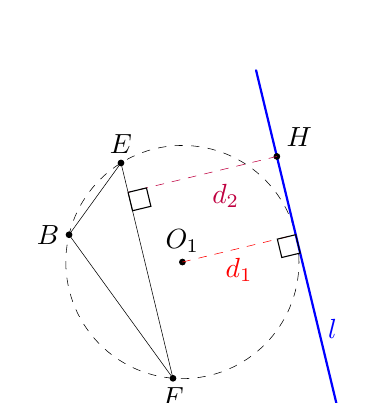
\begin{tikzpicture}[scale=1.2]
    % --- 1. 定義圓心 M, N 與半徑 ---
    \tkzDefPoint(-2,0){M}
    \tkzDefPoint(3,0){N}
    \def\rO{2}
    \def\rG{4}
    
    % --- 2. 定義直線 MN 上的 C, D (確保 C, M, N, D 順序) ---
    \tkzDefPoint(-2-\rO,0){C}
    \tkzDefPoint(3+\rG,0){D}
    
    % --- 3. 繪製兩圓 Omega, Gamma ---
    %\tkzDrawCircle[thick,black](M,C)
    %\tkzDrawCircle[thick,black](N,D)
    
    % --- 4. 求兩圓交點 A, B ---
    \tkzInterCC(M,C)(N,D) \tkzGetPoints{A}{B}
    
    % --- 5. 定義 P 為三角形 ACD 的外心 ---
    \tkzCircumCenter(A,C,D) \tkzGetPoint{P}
    %\tkzDrawCircle[dashed, cyan](P,A) % 繪製 ACD 的外接圓供參考
    %\tkzDrawArc[color=red, dashed](P,D)(C)
    % --- 6. 構造割線 AP 並求交點 E, F ---
    \tkzInterLC(A,P)(M,C) \tkzGetPoints{E}{A_tmp}
    \tkzInterLC(A,P)(N,D) \tkzGetPoints{A_tmp2}{F}
    
    % --- 7. 計算三角形 PMN 的垂心 H ---
    \tkzOrthoCenter(P,M,N) \tkzGetPoint{H}
    
    % --- 8. 繪製三角形 BEF 的外接圓 ---
    \tkzCircumCenter(B,E,F) \tkzGetPoint{O_1}
    \tkzDrawCircle[dashed, black](O_1,B)
    
    % --- 9. 繪製通過 H 且平行於 AP 的切線 l ---
    \tkzDefLine[parallel=through H](A,P) \tkzGetPoint{l_dir}
    \tkzDrawLine[blue, thick, add=0.1 and -0.7](H,l_dir)
    
    % --- 10. 繪製線段與標籤 ---
    %\tkzDrawLines[add=0.1 and 0.1](C,D)
    %\tkzDrawSegments(A,P P,M P,N A,B B,E B,F)
    %\tkzDrawPoints[fill=black](M,N,A,B,C,D,E,F,P,H)
    \tkzDrawPoints[fill=black](B,E,F,H,O_1)
    %\tkzLabelPoints[above](M,N)
    %\tkzLabelPoints[above left](C)
    %\tkzLabelPoints[above right](D,H)
    \tkzLabelPoints[above right](H)
    \tkzLabelPoints[left](B)
    %\tkzLabelPoints[above](A)
    %\tkzLabelPoints[below](P)
    \tkzLabelPoints[above](E)
    \tkzLabelPoints[below](F)
    \tkzLabelPoints[above](O_1)
    
    %\node at (-2-\rO*0.8,\rO*0.8) {$\Omega$};
    %\node at (3+\rG*0.8,\rG*0.8) {$\Gamma$};
    
    \coordinate (l_1) at ($(H)!0.2!(l_dir)$);
    \node[blue, right] at (l_1) {$l$};
    % 1. 找出 O1 在直線 (H, l_dir) 上的投影點（垂足），命名為 K
    \tkzDefPointBy[projection = onto H--l_dir](O_1) \tkzGetPoint{K}

    % 2. 繪製垂線段 O1K
    \tkzDrawSegment[color=red, dashed](O_1,K)

    % 3. 繪製直角符號
    \tkzMarkRightAngle[size=0.2](O_1,K,l_dir)

    \coordinate (d_1) at ($(O_1)!0.5!(K)$);
    \node[red, below] at (d_1) {$d_1$};
    \tkzDrawSegments(B,E B,F E,F)

     % 1. 找出 H 在直線 (E, F) 上的投影點（垂足），命名為 M
    \tkzDefPointBy[projection = onto E--F](H) \tkzGetPoint{M}

    % 2. 繪製垂線段 O1K
    \tkzDrawSegment[color=purple, dashed](H,M)

    % 3. 繪製直角符號
    \tkzMarkRightAngle[size=0.2](H,M,F)
    \coordinate (d_2) at ($(H)!0.5!(M)$);
    \node[purple, below right] at (d_2) {$d_2$};
  \end{tikzpicture}
\end{center}
現在把幾何圖的子圖放大，並記一對平行線$\left(EF,l\right)$之間的距離為$d_2$，則原命題等價於下方的命題一：
\begin{equation}
  d_1=R_1\Leftrightarrow d_2=R_1+\left\{O_1\text{到}EF\text{的距離}\right\}=R_1-R_1\cos{\angle{EBF}}
\end{equation}
同時，$d_2$ 的長度等於 $H$ 到 $EF$ 的距離。另一方面，$H$為$\triangle{BEF}$的垂心，且$P$在直線$EF$上，所以連結$HP$是必然的。
\begin{center}
  \begin{tikzpicture}[rotate=75, scale=1.2]
    % --- 1. 定義圓心 M, N 與半徑 ---
    \tkzDefPoint(-2,0){M}
    \tkzDefPoint(3,0){N}
    \def\rO{2}
    \def\rG{4}
    
    % --- 2. 定義直線 MN 上的 C, D (確保 C, M, N, D 順序) ---
    \tkzDefPoint(-2-\rO,0){C}
    \tkzDefPoint(3+\rG,0){D}
    
    % --- 3. 繪製兩圓 Omega, Gamma ---
    %\tkzDrawCircle[thick,black](M,C)
    %\tkzDrawCircle[thick,black](N,D)
    
    % --- 4. 求兩圓交點 A, B ---
    \tkzInterCC(M,C)(N,D) \tkzGetPoints{A}{B}
    
    % --- 5. 定義 P 為三角形 ACD 的外心 ---
    \tkzCircumCenter(A,C,D) \tkzGetPoint{P}
    %\tkzDrawCircle[dashed, cyan](P,A) % 繪製 ACD 的外接圓供參考
    %\tkzDrawArc[color=red, dashed](P,D)(C)
    % --- 6. 構造割線 AP 並求交點 E, F ---
    \tkzInterLC(A,P)(M,C) \tkzGetPoints{E}{A_tmp}
    \tkzInterLC(A,P)(N,D) \tkzGetPoints{A_tmp2}{F}
    
    % --- 7. 計算三角形 PMN 的垂心 H ---
    \tkzOrthoCenter(P,M,N) \tkzGetPoint{H}
    
    % --- 8. 繪製三角形 BEF 的外接圓 ---
    \tkzCircumCenter(B,E,F) \tkzGetPoint{O_1}
    \tkzDrawCircle[dashed, black](O_1,B)
    
    % --- 9. 繪製通過 H 且平行於 AP 的切線 l ---
    \tkzDefLine[parallel=through H](A,P) \tkzGetPoint{l_dir}
    \tkzDrawLine[blue, thick, add=0.1 and -0.7](H,l_dir)
    
    % --- 10. 繪製線段與標籤 ---
    %\tkzDrawLines[add=0.1 and 0.1](C,D)
    %\tkzDrawSegments(A,P P,M P,N A,B B,E B,F)
    %\tkzDrawPoints[fill=black](M,N,A,B,C,D,E,F,P,H)
    \tkzDrawPoints[fill=black](B,E,F,H,P)
    %\tkzLabelPoints[above](M,N)
    %\tkzLabelPoints[above left](C)
    %\tkzLabelPoints[above right](D,H)
    \tkzLabelPoints[above](H)
    \tkzLabelPoints[below](B)
    %\tkzLabelPoints[above](A)
    \tkzLabelPoints[below](P)
    \tkzLabelPoints[left](E)
    \tkzLabelPoints[below right](F)
    %\tkzLabelPoints[above](O_1)
    
    %\node at (-2-\rO*0.8,\rO*0.8) {$\Omega$};
    %\node at (3+\rG*0.8,\rG*0.8) {$\Gamma$};
    
    \coordinate (l_1) at ($(H)!0.2!(l_dir)$);
    \node[blue, above] at (l_1) {$l$};
    % 1. 找出 O1 在直線 (H, l_dir) 上的投影點（垂足），命名為 K
    %\tkzDefPointBy[projection = onto H--l_dir](O_1) \tkzGetPoint{K}

    % 2. 繪製垂線段 O1K
    %\tkzDrawSegment[color=red, dashed](O_1,K)

    % 3. 繪製直角符號
    %\tkzMarkRightAngle[size=0.2](O_1,K,l_dir)

    %\coordinate (d_1) at ($(O_1)!0.5!(K)$);
    %\node[red, below] at (d_1) {$d_1$};
    \tkzDrawSegments(B,E B,F E,P)
    \tkzDrawSegments[dashed](H,P)

     % 1. 找出 H 在直線 (E, F) 上的投影點（垂足），命名為 M
    \tkzDefPointBy[projection = onto E--F](H) \tkzGetPoint{M}

    % 2. 繪製垂線段 O1K
    \tkzDrawSegment[color=purple, dashed](H,M)

    % 3. 繪製直角符號
    \tkzMarkRightAngle[size=0.2](H,M,F)
    \coordinate (d_2) at ($(H)!0.5!(M)$);
    \node[purple, below right] at (d_2) {$d_2$};

\end{tikzpicture}
\end{center}
所以命題一等價於下方的命題二：
\begin{equation}
  HP\sin{\angle{HPE}}=d_2=R_1\left(1-\cos{\angle{EBF}}\right)
\end{equation}
現在只剩下$R_1$仍未計算出來，所以下一步就是計算$R_1$的長度。對$\triangle{BEF}$使用正弦定理可得：
\begin{equation}
  2R_1=\frac{BE}{\sin{\angle{BFE}}}\left(=\frac{BF}{\sin{\angle{BEF}}}\right)
\end{equation}
所以命題二等價於下方的命題三：
\begin{equation}
  HP\sin{\angle{HPE}}=\frac{BE}{2\sin{\angle{BFE}}}\left(1-\cos{\angle{EBF}}\right)
\end{equation}

下一步，我們需要把命題三中的各個量轉化成與$E,F$無關的量：
\begin{itemize}
  \item 因為$A,B$是圓$\Omega$與$\Gamma$的交點，所以$AB$是兩圓的公共弦，因此$AB\perp MN$。
  同時，$H$是$\triangle{PMN}$的垂心，所以$PH\perp MN$。由此可得 $AB\parallel PH$，所以$$\angle{HPE}=\angle{BAP}$$
  \item 記圓$\Omega$的半徑為$R_M$，對圓$\Omega$使用正弦定理：$$BE=2R_M\sin{\angle{BAE}}=2R_M\sin{\angle{BAP}}$$
  \item 在圓$\Gamma$中使用Angle Chasing：$\angle{BFE}=\angle{BFA}=\angle{BDA}$。記圓$\Gamma$的半徑為$R_N$，對圓$\Gamma$使用正弦定理：
  $$\sin{\angle{BFE}}=\sin{\angle{BDA}}=\frac{BA}{2R_N}$$
  \item $$\angle{EBF}=180^{\circ}-\angle{BEF}-\angle{BFE}=180^{\circ}-\angle{BEF}-\angle{BDA}$$
  在圓$\Gamma$中使用Angle Chasing：$$\angle{BEF}=\angle{BCA}$$
  所以有$$\angle{EBF}=180^{\circ}-\angle{BCA}-\angle{BDA}$$
  \iffalse
  利用圓周角定理可知
  $$\begin{cases}\angle{BCA}=\frac{1}{2}\angle{BMA}=\angle{AMN}\\ \angle{BDA}=\frac{1}{2}\angle{BNA}=\angle{ANM}\end{cases}$$
  因此
  $$\angle{EBF}=180^{\circ}-\angle{AMN}-\angle{ANM}=\angle{MAN}$$
  \fi
\end{itemize}
將上述結果代入命題三，可得命題四：
\begin{align}
  HP\sin{\angle{BAP}}&=\frac{2R_M\sin{\angle{BAP}}}{2\cdot\frac{BA}{2R_N}}
  \left[1-\cos{\left(180^{\circ}-\angle{BCA}-\angle{BDA}\right)}\right]\notag\\
  &=\frac{2R_MR_N\sin{\angle{BAP}}}{AB}\left[1+\cos{\left(\angle{BCA}+\angle{BDA}\right)}\right]
\end{align}
命題四兩邊都存在$\sin{\angle{BAP}}$，所以可以約去，得到命題五：
\begin{equation}
  HP=\frac{2R_MR_N}{AB}\left[1+\cos{\left(\angle{BCA}+\angle{BDA}\right)}\right]
\end{equation}
下一步，我們需要想辦法把$HP$的長度表示成與$H$無關的量，所以我把另一個幾何圖的子圖放大
\begin{center}
\begin{tikzpicture}[rotate=-90, scale=0.6]
    % --- 1. 定義圓心 M, N 與半徑 ---
    \tkzDefPoint(-2,0){M}
    \tkzDefPoint(3,0){N}
    \def\rO{2}
    \def\rG{4}
    
    % --- 2. 定義直線 MN 上的 C, D (確保 C, M, N, D 順序) ---
    \tkzDefPoint(-2-\rO,0){C}
    \tkzDefPoint(3+\rG,0){D}
    
    % --- 3. 繪製兩圓 Omega, Gamma ---
    %\tkzDrawCircle[thick,black](M,C)
    %\tkzDrawCircle[thick,black](N,D)
    
    % --- 4. 求兩圓交點 A, B ---
    \tkzInterCC(M,C)(N,D) \tkzGetPoints{A}{B}
    
    % --- 5. 定義 P 為三角形 ACD 的外心 ---
    \tkzCircumCenter(A,C,D) \tkzGetPoint{P}
    %\tkzDrawCircle[dashed, cyan](P,A) % 繪製 ACD 的外接圓供參考
    %\tkzDrawArc[color=red, dashed](P,D)(C)
    % --- 6. 構造割線 AP 並求交點 E, F ---
    \tkzInterLC(A,P)(M,C) \tkzGetPoints{E}{A_tmp}
    \tkzInterLC(A,P)(N,D) \tkzGetPoints{A_tmp2}{F}
    
    % --- 7. 計算三角形 PMN 的垂心 H ---
    \tkzOrthoCenter(P,M,N) \tkzGetPoint{H}
    
    % --- 10. 繪製線段與標籤 ---
    %\tkzDrawLines[add=0.1 and 0.1](C,D)
    \tkzDrawSegments(M,N P,N P,M)
    \tkzDrawPoints[fill=black](M,N,P,H)
    
    \tkzLabelPoints[right](M,N)
    \tkzLabelPoints[above left](H)
    \tkzLabelPoints[below](P)
    
    %\coordinate (l_1) at ($(H)!0.2!(l_dir)$);
    %\node[blue, right] at (l_1) {$l$};

\end{tikzpicture}
\end{center}
如果大家還記得「垂心-重心-外心」關係的話，很快就能得到：
$$
\overrightarrow{O_2H}=\overrightarrow{O_2P}+\overrightarrow{O_2M}+\overrightarrow{O_2N}
\Leftrightarrow\overrightarrow{PH}=\overrightarrow{O_2M}+\overrightarrow{O_2N}
$$
其中$O_2$為$\triangle{PMN}$的外心，為了讀者能更清晰地去計算，下圖為添加了$O_2$的幾何圖子圖：
\begin{center}
\begin{tikzpicture}[rotate=-90, scale=0.6]
    % --- 1. 定義圓心 M, N 與半徑 ---
    \tkzDefPoint(-2,0){M}
    \tkzDefPoint(3,0){N}
    \def\rO{2}
    \def\rG{4}
    
    % --- 2. 定義直線 MN 上的 C, D (確保 C, M, N, D 順序) ---
    \tkzDefPoint(-2-\rO,0){C}
    \tkzDefPoint(3+\rG,0){D}
    
    % --- 3. 繪製兩圓 Omega, Gamma ---
    %\tkzDrawCircle[thick,black](M,C)
    %\tkzDrawCircle[thick,black](N,D)
    
    % --- 4. 求兩圓交點 A, B ---
    \tkzInterCC(M,C)(N,D) \tkzGetPoints{A}{B}
    
    % --- 5. 定義 P 為三角形 ACD 的外心 ---
    \tkzCircumCenter(A,C,D) \tkzGetPoint{P}
    %\tkzDrawCircle[dashed, cyan](P,A) % 繪製 ACD 的外接圓供參考
    %\tkzDrawArc[color=red, dashed](P,D)(C)
    % --- 6. 構造割線 AP 並求交點 E, F ---
    \tkzInterLC(A,P)(M,C) \tkzGetPoints{E}{A_tmp}
    \tkzInterLC(A,P)(N,D) \tkzGetPoints{A_tmp2}{F}
    
    % --- 7. 計算三角形 PMN 的垂心 H ---
    \tkzOrthoCenter(P,M,N) \tkzGetPoint{H}
    \tkzCircumCenter(P,M,N) \tkzGetPoint{O_2}
    \tkzDrawCircle[dashed, black](O_2,M)
    % --- 10. 繪製線段與標籤 ---
    %\tkzDrawLines[add=0.1 and 0.1](C,D)
    \tkzDrawSegments(M,N P,N P,M)
    \tkzDrawSegments[dashed, black](O_2,M O_2,N)
    \tkzDrawPoints[fill=black](M,N,P,H,O_2)
    
    \tkzLabelPoints[right](M,N)
    \tkzLabelPoints[above left](H)
    \tkzLabelPoints[below](P)
    \tkzLabelPoints[below](O_2)
    
    %\coordinate (l_1) at ($(H)!0.2!(l_dir)$);
    %\node[blue, right] at (l_1) {$l$};

\end{tikzpicture}
\end{center}
記此外接圓半徑為$R_2$，由幾何關係可以算得
\begin{align*}
  HP&=\left|\overrightarrow{O_2M}+\overrightarrow{O_2N}\right|=2R_2\cos{\frac{\angle{MO_2N}}{2}}\\
  &=2R_2\cos{\angle{MPN}}=\frac{MN}{\sin{}\angle{MPN}}\cos{\angle{MPN}}\\
  &=MN\cot{\angle{MPN}}
\end{align*}
代入命題五可得
\begin{equation}
  MN\cot{\angle{MPN}}=\frac{2R_MR_N}{AB}\left[1+\cos{\left(\angle{BCA}+\angle{BDA}\right)}\right]
\end{equation}
現在整理當前的幾何圖
\begin{center}
\begin{tikzpicture}[scale=0.8]
    % --- 1. 定義圓心 M, N 與半徑 ---
    \tkzDefPoint(-2,0){M}
    \tkzDefPoint(3,0){N}
    \def\rO{2}
    \def\rG{4}
    
    % --- 2. 定義直線 MN 上的 C, D (確保 C, M, N, D 順序) ---
    \tkzDefPoint(-2-\rO,0){C}
    \tkzDefPoint(3+\rG,0){D}
    
    % --- 3. 繪製兩圓 Omega, Gamma ---
    \tkzDrawCircle[thick,black](M,C)
    \tkzDrawCircle[thick,black](N,D)
    
    % --- 4. 求兩圓交點 A, B ---
    \tkzInterCC(M,C)(N,D) \tkzGetPoints{A}{B}
    
    % --- 5. 定義 P 為三角形 ACD 的外心 ---
    \tkzCircumCenter(A,C,D) \tkzGetPoint{P}
    %\tkzDrawCircle[dashed, cyan](P,A) % 繪製 ACD 的外接圓供參考
    \tkzDrawArc[color=red, dashed](P,D)(C)
    
    % --- 10. 繪製線段與標籤 ---
    \tkzDrawLines[add=0.1 and 0.1](C,D)
    \tkzDrawSegments(A,P P,M P,N A,B)
    \tkzDrawPoints[fill=black](M,N,A,B,C,D,P)
    
    \tkzLabelPoints[above](M,N)
    \tkzLabelPoints[above left](C)
    \tkzLabelPoints[above right](D)
    \tkzLabelPoints[above left](B)
    \tkzLabelPoints[above](A)
    \tkzLabelPoints[below](P)
    
    \node at (-2-\rO*0.8,\rO*0.8) {$\Omega$};
    \node at (3+\rG*0.8,\rG*0.8) {$\Gamma$};
\end{tikzpicture}
\end{center}
下一步，我們需要把$\angle{MPN}$表示成與$P$無關的量，即把$P$點消去：

因為$P$為$\triangle{ACD}$的外心，而$M$為$\triangle{ACB}$的外心，所以直線$MP$為$AC$的中垂線。
同理，直線$NP$為$AD$的中垂線。

為了能夠更清楚地解釋，筆者再提取了幾何圖的子圖：
\begin{center}
  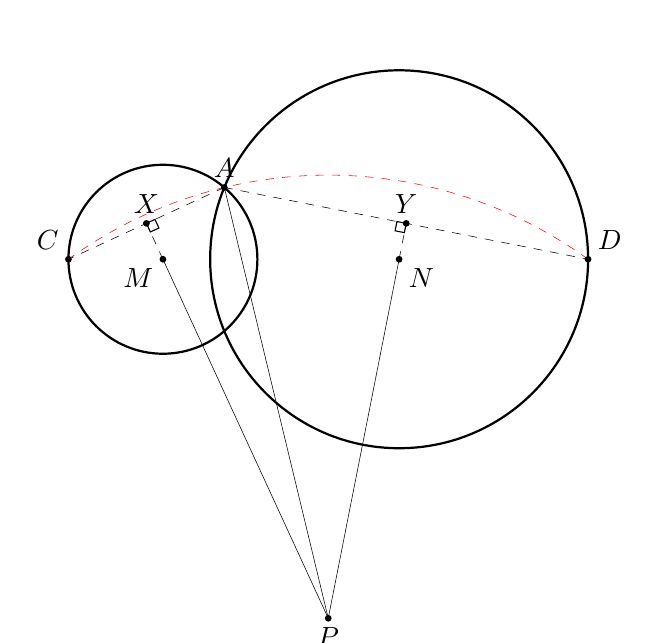
\begin{tikzpicture}[scale=0.6]
    % --- 1. 定義圓心 M, N 與半徑 ---
    \tkzDefPoint(-2,0){M}
    \tkzDefPoint(3,0){N}
    \def\rO{2}
    \def\rG{4}
    
    % --- 2. 定義直線 MN 上的 C, D (確保 C, M, N, D 順序) ---
    \tkzDefPoint(-2-\rO,0){C}
    \tkzDefPoint(3+\rG,0){D}
    
    % --- 3. 繪製兩圓 Omega, Gamma ---
    \tkzDrawCircle[thick,black](M,C)
    \tkzDrawCircle[thick,black](N,D)
    
    % --- 4. 求兩圓交點 A, B ---
    \tkzInterCC(M,C)(N,D) \tkzGetPoints{A}{B}
    
    % --- 5. 定義 P 為三角形 ACD 的外心 ---
    \tkzCircumCenter(A,C,D) \tkzGetPoint{P}
    %\tkzDrawCircle[dashed, cyan](P,A) % 繪製 ACD 的外接圓供參考
    \tkzDrawArc[color=red, dashed](P,D)(C)
    
    % 1. 求直線 MP 與 AC 的交點，命名為 Q
    \tkzInterLL(M,P)(A,C) \tkzGetPoint{X}
    \tkzInterLL(N,P)(A,D) \tkzGetPoint{Y}

    % --- 10. 繪製線段與標籤 ---
    %\tkzDrawLines[add=0.1 and 0.1](C,D)
    \tkzDrawSegments(A,P P,M P,N)
    \tkzDrawSegments[dashed](M,X A,C N,Y A,D)
    \tkzDrawPoints[fill=black](M,N,A,C,D,P,X,Y)
    
    \tkzLabelPoints[below left](M)
    \tkzLabelPoints[below right](N)
    \tkzLabelPoints[above left](C)
    \tkzLabelPoints[above right](D)
    \tkzLabelPoints[above](A)
    \tkzLabelPoints[below](P)
    \tkzLabelPoints[above](X,Y)

    \tkzMarkRightAngle[size=0.2](M,X,A)
    \tkzMarkRightAngle[size=0.2](N,Y,A)

  \end{tikzpicture}
\end{center}
記$PM$交$AC$於$X$，$PN$交$AD$於$Y$，由$PM\perp AC$和$PN\perp AD$可知$A,X,P,Y$四點共圖，所以
$$\angle{MPN}=\angle{XPY}=180^{\circ}-\angle{XAY}=180^{\circ}-\angle{CAD}$$
代入至命題五可得：
\begin{equation}
  \frac{2R_MR_N}{AB}\left[1+\cos{\left(\angle{BCA}+\angle{BDA}\right)}\right]
  =MN\cot{\left(180^{\circ}-\angle{CAD}\right)}=-MN\cot{\angle{CAD}}
\end{equation}
現在整理當前的幾何圖
\begin{center}
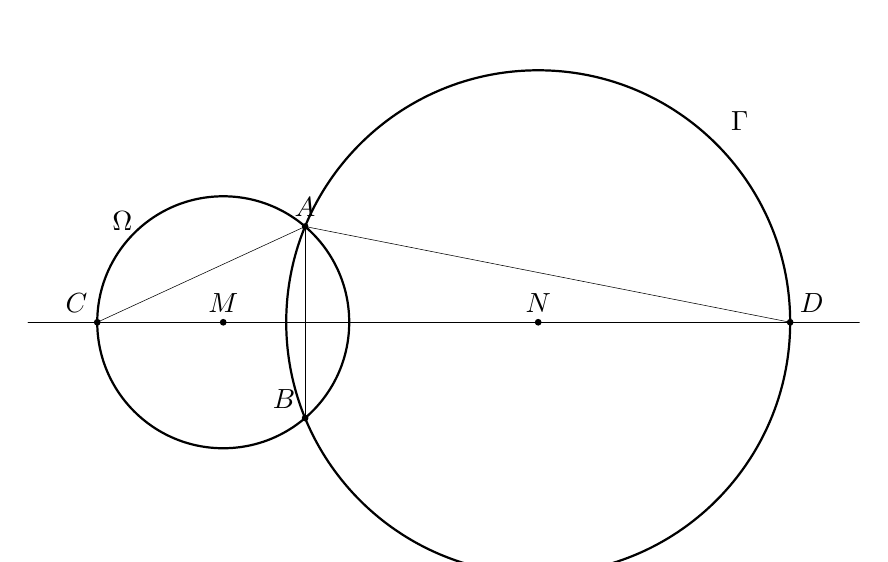
\begin{tikzpicture}[scale=0.8]
    % --- 1. 定義圓心 M, N 與半徑 ---
    \tkzDefPoint(-2,0){M}
    \tkzDefPoint(3,0){N}
    \def\rO{2}
    \def\rG{4}
    
    % --- 2. 定義直線 MN 上的 C, D (確保 C, M, N, D 順序) ---
    \tkzDefPoint(-2-\rO,0){C}
    \tkzDefPoint(3+\rG,0){D}
    
    % --- 3. 繪製兩圓 Omega, Gamma ---
    \tkzDrawCircle[thick,black](M,C)
    \tkzDrawCircle[thick,black](N,D)
    
    % --- 4. 求兩圓交點 A, B ---
    \tkzInterCC(M,C)(N,D) \tkzGetPoints{A}{B}
    
    % --- 10. 繪製線段與標籤 ---
    \tkzDrawLines[add=0.1 and 0.1](C,D)
    \tkzDrawSegments(A,B C,A A,D)
    \tkzDrawPoints[fill=black](M,N,A,B,C,D)
    
    \tkzLabelPoints[above](M,N)
    \tkzLabelPoints[above left](C)
    \tkzLabelPoints[above right](D)
    \tkzLabelPoints[above left](B)
    \tkzLabelPoints[above](A)
    
    \node at (-2-\rO*0.8,\rO*0.8) {$\Omega$};
    \node at (3+\rG*0.8,\rG*0.8) {$\Gamma$};
\end{tikzpicture}
\end{center}
下一步，我們要消去$C,D$兩點：
利用圓周角定理可知
  $$\begin{cases}\angle{BCA}=\frac{1}{2}\angle{BMA}=\angle{AMN}\\ \angle{BDA}=\frac{1}{2}\angle{BNA}=\angle{ANM}\end{cases}$$
所以有
$$
\angle{BCA}+\angle{BDA}=\angle{AMN}+\angle{ANM}=180^{\circ}-\angle{MAN}
$$
另一方面
\begin{align*}
  \angle{CAD}&=\angle{MAN}+\angle{CAM}+\angle{DAN}\\
  &=\angle{MAN}+\angle{MAC}+\angle{NDA}\\
  &=\angle{MAN}+\frac{1}{2}\left(\angle{BCA}+\angle{BDA}\right)\\
  &=\angle{MAN}+\frac{1}{2}\left(180^{\circ}-\angle{MAN}\right)\\
  &=90^{\circ}+\frac{1}{2}\angle{MAN}
\end{align*}
因此命題五等價於下方的命題六：
\begin{align}
  &\frac{2R_MR_N}{AB}\left[1+\cos{\left(180^{\circ}-\angle{MAN}\right)}\right]
  =-MN\cot{\left(90^{\circ}+\frac{1}{2}\angle{MAN}\right)}\notag\\
  \Leftrightarrow\quad&\frac{2R_MR_N}{AB}\left(1-\cos{\angle{MAN}}\right)
  =MN\tan{\frac{\angle{MAN}}{2}}\notag\\
  \Leftrightarrow\quad&\frac{2R_MR_N}{AB}\cdot2\sin^2{\frac{\angle{MAN}}{2}}=MN\cdot\tan{\frac{\angle{MAN}}{2}}\notag\\
  \Leftrightarrow\quad&\frac{2R_MR_N}{AB}\cdot2\sin{\frac{\angle{MAN}}{2}}\cos{\frac{\angle{MAN}}{2}}=MN\notag\\
  \Leftrightarrow\quad&\frac{2R_MR_N}{AB}\sin{\angle{MAN}}=MN\notag\\
  \Leftrightarrow\quad&2R_MR_N\sin{\angle{MAN}}=MN\cdot AB
\end{align}
現在整理當前的幾何圖
\begin{center}
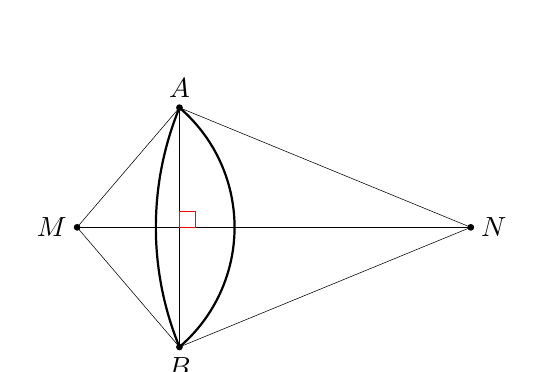
\begin{tikzpicture}[scale=1]
    % --- 1. 定義圓心 M, N 與半徑 ---
    \tkzDefPoint(-2,0){M}
    \tkzDefPoint(3,0){N}
    \def\rO{2}
    \def\rG{4}
    
    % --- 2. 定義直線 MN 上的 C, D (確保 C, M, N, D 順序) ---
    \tkzDefPoint(-2-\rO,0){C}
    \tkzDefPoint(3+\rG,0){D}
    
    % --- 4. 求兩圓交點 A, B ---
    \tkzInterCC(M,C)(N,D) \tkzGetPoints{A}{B}

        % --- 3. 繪製兩圓 Omega, Gamma ---
    \tkzDrawArc[thick,black](M,B)(A)
    \tkzDrawArc[thick,black](N,A)(B)
    
    % --- 10. 繪製線段與標籤 ---
    %\tkzDrawLines[add=0.1 and 0.1](C,D)
    \tkzDrawSegments(A,B A,M A,N B,M B,N M,N)
    \tkzDrawPoints[fill=black](M,N,A,B)
    
    \tkzLabelPoints[left](M)
    \tkzLabelPoints[right](N)
    \tkzLabelPoints[below](B)
    \tkzLabelPoints[above](A)

        % 1. 求直線 MP 與 AC 的交點，命名為 Q
    \tkzInterLL(M,N)(A,B) \tkzGetPoint{K}
    \tkzMarkRightAngle[size=0.2, red](A,K,N)
\end{tikzpicture}
\end{center}
因為 $MN\perp AB$，所以
\begin{equation}
  \left[AMBN\right]=\frac{1}{2}MN\cdot AB\label{eq:Area_AMBN_1}
\end{equation}
另一方面，易知 $\triangle{AMN}\cong\triangle{BMN}$，所以
\begin{align}
  \left[AMBN\right]&=\left[\triangle{AMN}\right]+\left[\triangle{BMN}\right]\notag\\
  &=2\left[\triangle{AMN}\right]\notag\\
  &=AM\cdot AN\sin{\angle{MAN}}\notag\\
  &=R_MR_N\sin{\angle{MAN}}\label{eq:Area_AMBN_2}
\end{align}
聯立式\eqref{eq:Area_AMBN_1}與式\eqref{eq:Area_AMBN_2}可得
\begin{align}
  &\frac{1}{2}MN\cdot AB=R_MR_N\sin{\angle{MAN}}\notag\\
  \Leftrightarrow\quad&2R_MR_N\sin{\angle{MAN}}=MN\cdot AB
\end{align}
由此可證得命題六成立，即原命題成立。
\end{mybox}

\newpage

\begin{mybox}[問題2]{4em}{1em}
    設四邊形$ABCD$是梯形，$AB\parallel CD$且$AB<CD$。直線$AD$和$BC$交於點$P$。$\triangle{ABC}$上的一點$X\neq C$滿足$PX=PC$，$\triangle{ABD}$上的一點$Y\neq D$滿足$PY=PD$
    直線$AX$與$BY$交於點$Q$。\\[0.5em]
    求證：$PQ\parallel AB$
    \begin{center}
      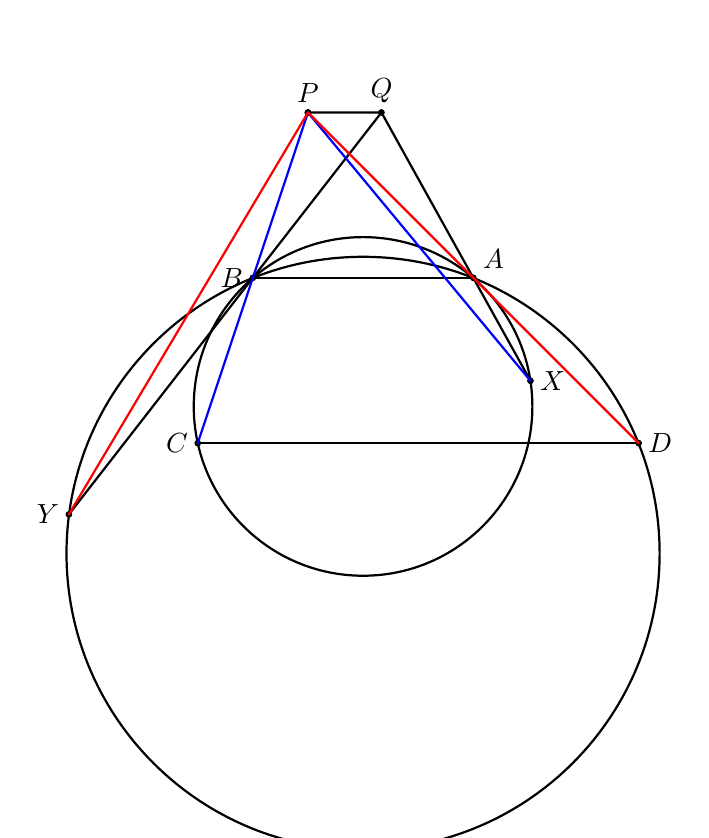
\begin{tikzpicture}[scale=0.7]
      % 1. 滿足 AB || CD 且 AB < CD，且非等腰
      \tkzDefPoint(2,3){A}
      \tkzDefPoint(-2,3){B}
      \tkzDefPoint(-3,0){C}
      \tkzDefPoint(5,0){D}
      
      % 2. 找到 AD 與 BC 的交點 P
      \tkzInterLL(A,D)(B,C) \tkzGetPoint{P}

      % 3. 找到三角形 ABC 和 ABD 的外心
      \tkzCircumCenter(A,B,C) \tkzGetPoint{O_1}
      \tkzCircumCenter(A,B,D) \tkzGetPoint{O_2}

      % 4. 找到C關於O_1P的對稱點X
      \tkzInterCC(O_1,C)(P,C) \tkzGetPoints{C_tmp}{X}
      % 5. 找到D關於O_2P的對稱點Y
      \tkzInterCC(O_2,D)(P,D) \tkzGetPoints{Y}{D_tmp}

      % 6. 繪製三角形 ABC 和 ABD 的外接圓
      \tkzDrawCircle[black,thick](O_1,A)
      \tkzDrawCircle[black,thick](O_2,A)

      % 7. 找到 AX 與 BY 的交點 Q
      \tkzInterLL(A,X)(B,Y) \tkzGetPoint{Q}

      \tkzDrawPoints[fill=black](A,B,C,D,P,X,Y,P,Q)
      \tkzLabelPoints[right](D)
      \tkzLabelPoints[above right](A)
      \tkzLabelPoints[left](B,C)
      \tkzLabelPoints[above](P)
      \tkzLabelPoints[above](Q)
      \tkzLabelPoints[right](X)
      \tkzLabelPoints[left](Y)
      \tkzDrawSegments[black, thick](A,B C,D P,Q X,Q Y,Q)
      \tkzDrawSegments[blue, thick](P,X P,C)
      \tkzDrawSegments[red, thick](P,Y P,D)
    \end{tikzpicture}
    \end{center}
\end{mybox}
\newpage
\begin{mybox}{4em}{1em}
  要證明兩直線平行，方法不外乎以下幾種：
  \begin{enumerate}[label=(\arabic*)]
    \item 找到相等的同位角、內錯角
    \item 找到互補的同旁內角
    \item 向量平行
    \item 找到兩點（兩個點同一在直線上或分別在兩條直線都可）到另一條直線的距離相等
  \end{enumerate}
  如果要用第(1)種或第(2)種方法，
  那麼至少要研究 $\angle{PQA}$、$\angle{PQB}$、
  $\angle{QPA}$和$\angle{QPB}$ 之間的其中一個角。
  因為這些角都直接涉及到直線$PQ$，所以很難去轉換這些角。\\

  要用第(3)種方法，其困難在於寫出交點向量。
  非常不幸地，本題中含有大量交點，而且是圓與圓的交點，所以此方法亦不適用。\\

  要用第(4)種方法，
  可以嘗試以「$P$到$AB$的距離$d_{P,AB}$等於$Q$到$AB$的距離$d_{Q,AB}$」作為切入點。
  同時，因為$AB\parallel CD$，所以若原命題得證，則必定有「$P$到$CD$的距離$d_{P,CD}$等於$Q$到$AB$的距離$d_{Q,CD}$」成立。
  
  一般如果題目已知存在一對平行線，則最好把要論證的「數值」由「角度、長度、面積」變成「比值」，因為這樣可以配合相似三角形得到更多幾何關係。
  \begin{center}
      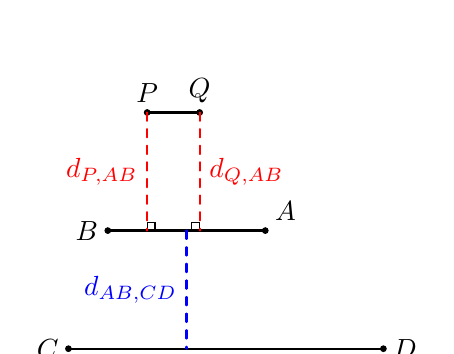
\begin{tikzpicture}[scale=0.5]
      % 1. 滿足 AB || CD 且 AB < CD，且非等腰
      \tkzDefPoint(2,3){A}
      \tkzDefPoint(-2,3){B}
      \tkzDefPoint(-3,0){C}
      \tkzDefPoint(5,0){D}
      
      % 2. 找到 AD 與 BC 的交點 P
      \tkzInterLL(A,D)(B,C) \tkzGetPoint{P}

      % 3. 找到三角形 ABC 和 ABD 的外心
      \tkzCircumCenter(A,B,C) \tkzGetPoint{O_1}
      \tkzCircumCenter(A,B,D) \tkzGetPoint{O_2}

      % 4. 找到C關於O_1P的對稱點X
      \tkzInterCC(O_1,C)(P,C) \tkzGetPoints{C_tmp}{X}
      % 5. 找到D關於O_2P的對稱點Y
      \tkzInterCC(O_2,D)(P,D) \tkzGetPoints{Y}{D_tmp}

      % 6. 繪製三角形 ABC 和 ABD 的外接圓
      %\tkzDrawCircle[black,thick](O_1,A)
      %\tkzDrawCircle[black,thick](O_2,A)

      % 7. 找到 AX 與 BY 的交點 Q
      \tkzInterLL(A,X)(B,Y) \tkzGetPoint{Q}

      \tkzDrawPoints[fill=black](A,B,C,D,P,Q)
      \tkzLabelPoints[right](D)
      \tkzLabelPoints[above right](A)
      \tkzLabelPoints[left](B,C)
      \tkzLabelPoints[above](P)
      \tkzLabelPoints[above](Q)
      %\tkzLabelPoints[right](X)
      %\tkzLabelPoints[left](Y)
      \tkzDrawSegments[black, thick](A,B C,D P,Q)
      %\tkzDrawSegments[blue, thick](P,X P,C)
      %\tkzDrawSegments[red, thick](P,Y P,D)

        % 1. 找出 O1 在直線 (H, l_dir) 上的投影點（垂足），命名為 K
        \tkzDefPointBy[projection = onto B--A](P) \tkzGetPoint{P_1}
        \tkzDefPointBy[projection = onto B--A](Q) \tkzGetPoint{Q_1}
        %\tkzDefPointBy[projection = onto C--D](P) \tkzGetPoint{P_2}
        %\tkzDefPointBy[projection = onto C--D](Q) \tkzGetPoint{Q_2}

        % 2. 繪製垂線段 O1K
        \tkzDrawSegment[color=red, dashed](P,P_1)
        \tkzDrawSegment[color=red, dashed](Q,Q_1)

        % 3. 繪製直角符號
        \tkzMarkRightAngle[size=0.2](P,P_1,A)
        %\tkzMarkRightAngle[size=0.2](P,P_2,D)
        \tkzMarkRightAngle[size=0.2](Q,Q_1,B)
        %\tkzMarkRightAngle[size=0.2](Q,Q_2,C)

        \coordinate (d_ABCD_1) at ($(B)!0.5!(A)$);
        \tkzDefPointBy[projection = onto C--D](d_ABCD_1) \tkzGetPoint{d_ABCD_2}
        \tkzDrawSegment[color=blue, dashed, thick](d_ABCD_1,d_ABCD_2)
        \tkzDrawSegment[color=red, dashed, thick](P,P_1)
        \tkzDrawSegment[color=red, dashed, thick](Q,Q_1)
        \node[blue, left] at ($(d_ABCD_1)!0.5!(d_ABCD_2)$) {$d_{AB,CD}$};
        \node[red, left] at ($(P)!0.5!(P_1)$) {$d_{P,AB}$};
        \node[red, right] at ($(Q)!0.5!(Q_1)$) {$d_{Q,AB}$};
    \end{tikzpicture}
  \end{center}
  
  提取出原幾何圖的子圖。顯然，當原命題成立時，「$d_{P,AB}:d_{P,CD}=d_{Q,AB}:d_{Q,CD}$」也必定成立。

  注意，題中的一對平行線$AB$和$CD$之間的距離$d_{AB,CD}$是一個「定值」。經過以下的等價變換
  \begin{align*}
    d_{P,AB}:d_{P,CD}=d_{Q,AB}:d_{Q,CD}\Leftrightarrow\quad& \frac{d_{P,CD}}{d_{P,AB}}=\frac{d_{Q,CD}}{d_{Q,AB}}\\ 
    \Leftrightarrow\quad& \frac{d_{P,CD}}{d_{P,AB}}-1=\frac{d_{Q,CD}}{d_{Q,AB}}-1\\ 
    \Leftrightarrow\quad& \frac{d_{AB,CD}}{d_{P,AB}}=\frac{d_{AB,CD}}{d_{Q,AB}}\\ 
    \Leftrightarrow\quad& d_{P,AB}=d_{Q,AB}\Rightarrow\quad PQ\parallel AB
  \end{align*}

  所以原命題等價於以下的命題一：
  \begin{equation}
    PQ\parallel AB\Leftrightarrow\frac{d_{P,AB}}{d_{P,CD}}=\frac{d_{Q,AB}}{d_{Q,CD}}\label{eq:p2_s1}
  \end{equation}

  \begin{center}
      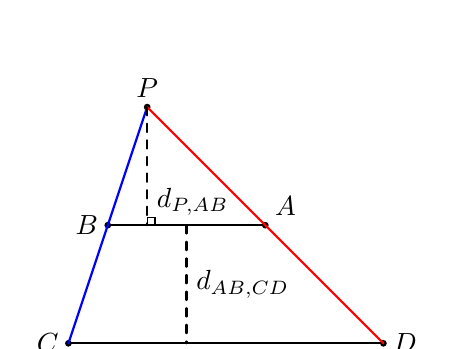
\begin{tikzpicture}[scale=0.5]
      % 1. 滿足 AB || CD 且 AB < CD，且非等腰
      \tkzDefPoint(2,3){A}
      \tkzDefPoint(-2,3){B}
      \tkzDefPoint(-3,0){C}
      \tkzDefPoint(5,0){D}
      
      % 2. 找到 AD 與 BC 的交點 P
      \tkzInterLL(A,D)(B,C) \tkzGetPoint{P}

      % 3. 找到三角形 ABC 和 ABD 的外心
      %\tkzCircumCenter(A,B,C) \tkzGetPoint{O_1}
      %\tkzCircumCenter(A,B,D) \tkzGetPoint{O_2}

      % 4. 找到C關於O_1P的對稱點X
      %\tkzInterCC(O_1,C)(P,C) \tkzGetPoints{C_tmp}{X}
      % 5. 找到D關於O_2P的對稱點Y
      %\tkzInterCC(O_2,D)(P,D) \tkzGetPoints{Y}{D_tmp}

      % 6. 繪製三角形 ABC 和 ABD 的外接圓
      %\tkzDrawCircle[black,thick](O_1,A)
      %\tkzDrawCircle[black,thick](O_2,A)

      % 7. 找到 AX 與 BY 的交點 Q
      %\tkzInterLL(A,X)(B,Y) \tkzGetPoint{Q}

      \tkzDrawPoints[fill=black](A,B,C,D,P)
      \tkzLabelPoints[right](D)
      \tkzLabelPoints[above right](A)
      \tkzLabelPoints[left](B,C)
      \tkzLabelPoints[above](P)
      %\tkzLabelPoints[above](Q)
      %\tkzLabelPoints[right](X)
      %\tkzLabelPoints[left](Y)
      \tkzDrawSegments[black, thick](A,B C,D)
      \tkzDrawSegments[blue, thick](P,C)
      \tkzDrawSegments[red, thick](P,D)

        % 1. 找出 O1 在直線 (H, l_dir) 上的投影點（垂足），命名為 K
        \tkzDefPointBy[projection = onto B--A](P) \tkzGetPoint{P_1}
        %\tkzDefPointBy[projection = onto B--A](Q) \tkzGetPoint{Q_1}
        %\tkzDefPointBy[projection = onto C--D](P) \tkzGetPoint{P_2}
        %\tkzDefPointBy[projection = onto C--D](Q) \tkzGetPoint{Q_2}

        % 2. 繪製垂線段 O1K
        \tkzDrawSegment[color=red, dashed](P,P_1)
        %\tkzDrawSegment[color=red, dashed](Q,Q_1)

        % 3. 繪製直角符號
        \tkzMarkRightAngle[size=0.2](P,P_1,A)
        %\tkzMarkRightAngle[size=0.2](P,P_2,D)
        %\tkzMarkRightAngle[size=0.2](Q,Q_1,B)
        %\tkzMarkRightAngle[size=0.2](Q,Q_2,C)

        \coordinate (d_ABCD_1) at ($(B)!0.5!(A)$);
        \tkzDefPointBy[projection = onto C--D](d_ABCD_1) \tkzGetPoint{d_ABCD_2}
        \tkzDrawSegment[color=black, dashed, thick](d_ABCD_1,d_ABCD_2)
        \tkzDrawSegment[color=black, dashed, thick](P,P_1)
        %\tkzDrawSegment[color=red, dashed, thick](Q,Q_1)
        \node[black, right] at ($(d_ABCD_1)!0.5!(d_ABCD_2)$) {$d_{AB,CD}$};
        \node[black, right] at ($(P)!0.8!(P_1)$) {$d_{P,AB}$};
        %\node[red, right] at ($(Q)!0.5!(Q_1)$) {$d_{Q,AB}$};
    \end{tikzpicture}
  \end{center}

  第一步，研究 $d_{P,AB}:d_{P,CD}$：
  
  因為$AB\parallel CD$，所以$\triangle{PBA}$和$\triangle{PCD}$是位似三角形，即有
  \begin{equation}
    \frac{d_{P,AB}}{d_{P,CD}}=\frac{PA}{PD}=\frac{PB}{PC}=\frac{BA}{CD}\label{eq:p2_s1-1}
  \end{equation}
  (\ref{eq:p2_s1-1})式中我們選擇$BA/CD$的值，因為此表達式上只存在$A,B,C,D$四點，是「最簡形式」。所以命題一等價於以下的命題二：
  \begin{equation}
    \frac{d_{Q,AB}}{d_{Q,CD}}=\frac{BA}{CD}\label{eq:p2_s2}
  \end{equation}
  留意到(\ref{eq:p2_s2})式中包含 $A,B,C,D,Q$ 五點。在原幾何圖中，已知線段已經連成了$\triangle{QAB}$，而命題二又與$CD$有關，所以我們需要令射線$QB$和$QA$與直線$CD$產生聯繫才可。

  第二步，研究 $d_{Q,AB}:d_{Q,CD}$：

  \begin{center}
      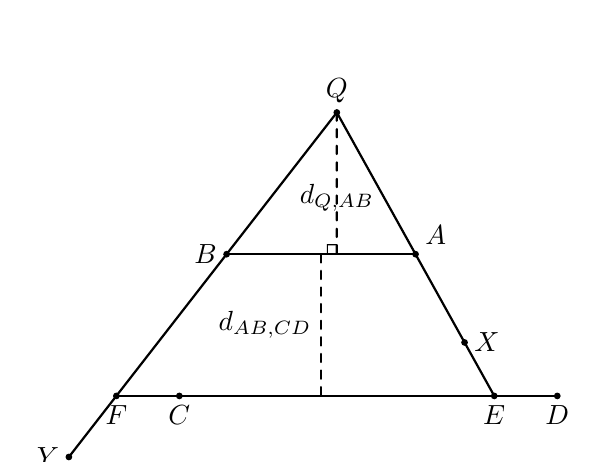
\begin{tikzpicture}[scale=0.6]
      % 1. 滿足 AB || CD 且 AB < CD，且非等腰
      \tkzDefPoint(2,3){A}
      \tkzDefPoint(-2,3){B}
      \tkzDefPoint(-3,0){C}
      \tkzDefPoint(5,0){D}
      
      % 2. 找到 AD 與 BC 的交點 P
      \tkzInterLL(A,D)(B,C) \tkzGetPoint{P}

      % 3. 找到三角形 ABC 和 ABD 的外心
      \tkzCircumCenter(A,B,C) \tkzGetPoint{O_1}
      \tkzCircumCenter(A,B,D) \tkzGetPoint{O_2}

      % 4. 找到C關於O_1P的對稱點X
      \tkzInterCC(O_1,C)(P,C) \tkzGetPoints{C_tmp}{X}
      % 5. 找到D關於O_2P的對稱點Y
      \tkzInterCC(O_2,D)(P,D) \tkzGetPoints{Y}{D_tmp}

      % 6. 繪製三角形 ABC 和 ABD 的外接圓
      %\tkzDrawCircle[black,thick](O_1,A)
      %\tkzDrawCircle[black,thick](O_2,A)

      % 7. 找到 AX 與 BY 的交點 Q
      \tkzInterLL(A,X)(B,Y) \tkzGetPoint{Q}
      \tkzInterLL(A,X)(C,D) \tkzGetPoint{E}
      \tkzInterLL(B,Y)(C,D) \tkzGetPoint{F}

      \tkzDrawPoints[fill=black](A,B,C,D,E,F,Q,X,Y)
      %\tkzLabelPoints[right](D)
      \tkzLabelPoints[above right](A)
      \tkzLabelPoints[left](B)
      \tkzLabelPoints[below](E,F,C,D)
      %\tkzLabelPoints[above](P)
      \tkzLabelPoints[above](Q)
      \tkzLabelPoints[right](X)
      \tkzLabelPoints[left](Y)
      \tkzDrawSegments[black, thick](A,B F,D Q,E Q,Y)
      %\tkzDrawSegments[blue, thick](P,X P,C)
      %\tkzDrawSegments[red, thick](P,Y P,D)

              % 1. 找出 O1 在直線 (H, l_dir) 上的投影點（垂足），命名為 K
        %\tkzDefPointBy[projection = onto B--A](P) \tkzGetPoint{P_1}
        \tkzDefPointBy[projection = onto B--A](Q) \tkzGetPoint{Q_1}
        %\tkzDefPointBy[projection = onto C--D](P) \tkzGetPoint{P_2}
        %\tkzDefPointBy[projection = onto C--D](Q) \tkzGetPoint{Q_2}

        % 2. 繪製垂線段 O1K
        %\tkzDrawSegment[color=red, dashed](P,P_1)
        \tkzDrawSegment[color=red, dashed](Q,Q_1)

        % 3. 繪製直角符號
        %\tkzMarkRightAngle[size=0.2](P,P_1,A)
        %\tkzMarkRightAngle[size=0.2](P,P_2,D)
        \tkzMarkRightAngle[size=0.2](Q,Q_1,B)
        %\tkzMarkRightAngle[size=0.2](Q,Q_2,C)

        \coordinate (d_ABCD_1) at ($(B)!0.5!(A)$);
        \tkzDefPointBy[projection = onto C--D](d_ABCD_1) \tkzGetPoint{d_ABCD_2}
        \tkzDrawSegment[color=black, dashed, thick](d_ABCD_1,d_ABCD_2)
        %\tkzDrawSegment[color=red, dashed, thick](P,P_1)
        \tkzDrawSegment[color=black, dashed, thick](Q,Q_1)
        \node[black, left] at ($(d_ABCD_1)!0.5!(d_ABCD_2)$) {$d_{AB,CD}$};
        %\node[red, left] at ($(P)!0.5!(P_1)$) {$d_{P,AB}$};
        \node[black] at ($(Q)!0.6!(Q_1)$) {$d_{Q,AB}$};
    \end{tikzpicture}
  \end{center}
  作直線$AX$與直線$CD$的交點為$E$，直線$BY$與直線$CD$的交點為$F$。\textcolor{gray}{（溫馨提示：雖然直線$AX$和直線$QA$是同一條，但是為了可以逐步消去$Q$點，在解答過程中亦盡量減少出現不出現的$Q$點；直線$BY$同理）}
  因為$AB\parallel CD$，即$AB\parallel EF$，所以$\triangle{QBA}$和$\triangle{QFE}$也是位似三角形，即有
  \begin{equation}
    \frac{d_{Q,AB}}{d_{Q,CD}}=\frac{QA}{QE}=\frac{QB}{QF}=\frac{BA}{FE}\label{eq:p2_s2-1}
  \end{equation}
  與第一步的情況一樣，我們選擇$BA/FE$的值，所以命題二等價於以下的命題三：
  \begin{equation}
    \frac{BA}{FE}=\frac{BA}{CD}\Leftrightarrow FE=CD\Leftrightarrow FC=ED\label{eq:p2_s3}
  \end{equation}
  至此，我們成功消去$Q$點，整理當前的幾何圖：
  \begin{center}
      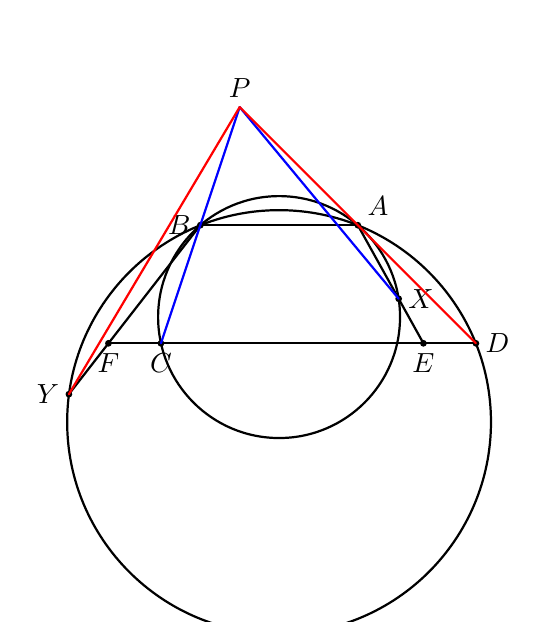
\begin{tikzpicture}[scale=0.5]
      % 1. 滿足 AB || CD 且 AB < CD，且非等腰
      \tkzDefPoint(2,3){A}
      \tkzDefPoint(-2,3){B}
      \tkzDefPoint(-3,0){C}
      \tkzDefPoint(5,0){D}
      
      % 2. 找到 AD 與 BC 的交點 P
      \tkzInterLL(A,D)(B,C) \tkzGetPoint{P}

      % 3. 找到三角形 ABC 和 ABD 的外心
      \tkzCircumCenter(A,B,C) \tkzGetPoint{O_1}
      \tkzCircumCenter(A,B,D) \tkzGetPoint{O_2}

      % 4. 找到C關於O_1P的對稱點X
      \tkzInterCC(O_1,C)(P,C) \tkzGetPoints{C_tmp}{X}
      % 5. 找到D關於O_2P的對稱點Y
      \tkzInterCC(O_2,D)(P,D) \tkzGetPoints{Y}{D_tmp}

      % 6. 繪製三角形 ABC 和 ABD 的外接圓
      \tkzDrawCircle[black,thick](O_1,A)
      \tkzDrawCircle[black,thick](O_2,A)

      % 7. 找到 AX 與 BY 的交點 Q
      %\tkzInterLL(A,X)(B,Y) \tkzGetPoint{Q}
      \tkzInterLL(A,X)(C,D) \tkzGetPoint{E}
      \tkzInterLL(B,Y)(C,D) \tkzGetPoint{F}

      \tkzDrawPoints[fill=black](A,B,C,D,E,F,X,Y)
      %\tkzLabelPoints[below left](C)
      \tkzLabelPoints[above right](A)
      \tkzLabelPoints[left](B)
      \tkzLabelPoints[below](E,F,C)
      \tkzLabelPoints[above](P)
      %\tkzLabelPoints[above](Q)
      \tkzLabelPoints[right](X,D)
      \tkzLabelPoints[left](Y)
      \tkzDrawSegments[black, thick](A,B F,D A,E B,Y)
      \tkzDrawSegments[blue, thick](P,X P,C)
      \tkzDrawSegments[red, thick](P,Y P,D)
    \end{tikzpicture}
  \end{center}

  第三步，歸類思維：

  (\ref{eq:p2_s3})式中的線段$FC$和$ED$沒有公共端點，無法簡單地形成比值關係，所以需要把目光投向「其他上層點」。\\

  注意到，$E$點是直線$AX$與$CD$相交而得，撇除初始點$A,C,D$後，會發現$E$點是受$X$點影響的。
  $X$點是由$C$點經過一些對稱變換而生成，且在$\triangle{ABC}$上，所以在腦海中可以生成一個「C類」，C類包含$\triangle{ABC}$、$\triangle{ABC}$的外接圓、$X$、$E$。

  同理，另一個就是「D類」，D類包含$\triangle{ABD}$、$\triangle{ABD}$的外接圓、$Y$、$F$。

  現在命題三中的兩線段$FC$和$ED$，明顯使兩個種類產生了糾纏，使得解題難度增高。我們需要做的，就是把兩個種類的糾纏部分拆開。
  \begin{center}
      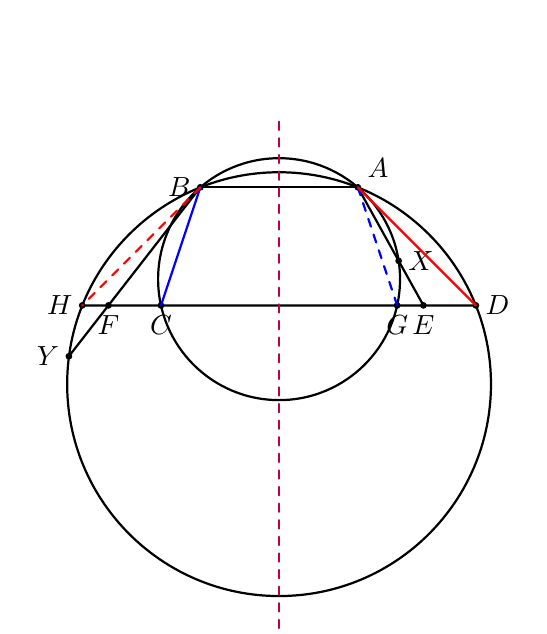
\begin{tikzpicture}[scale=0.5]
      % 1. 滿足 AB || CD 且 AB < CD，且非等腰
      \tkzDefPoint(2,3){A}
      \tkzDefPoint(-2,3){B}
      \tkzDefPoint(-3,0){C}
      \tkzDefPoint(5,0){D}
      
      % 2. 找到 AD 與 BC 的交點 P
      \tkzInterLL(A,D)(B,C) \tkzGetPoint{P}

      % 3. 找到三角形 ABC 和 ABD 的外心
      \tkzCircumCenter(A,B,C) \tkzGetPoint{O_1}
      \tkzCircumCenter(A,B,D) \tkzGetPoint{O_2}

      % 4. 找到C關於O_1P的對稱點X
      \tkzInterCC(O_1,C)(P,C) \tkzGetPoints{C_tmp}{X}
      % 5. 找到D關於O_2P的對稱點Y
      \tkzInterCC(O_2,D)(P,D) \tkzGetPoints{Y}{D_tmp}

      % 6. 繪製三角形 ABC 和 ABD 的外接圓
      \tkzDrawCircle[black,thick](O_1,A)
      \tkzDrawCircle[black,thick](O_2,A)

      % 7. 找到 AX 與 BY 的交點 Q
      %\tkzInterLL(A,X)(B,Y) \tkzGetPoint{Q}
      \tkzInterLL(A,X)(C,D) \tkzGetPoint{E}
      \tkzInterLL(B,Y)(C,D) \tkzGetPoint{F}
      \tkzInterLC(C,D)(O_1,A) \tkzGetPoints{C_tmp}{G}
      \tkzInterLC(C,D)(O_2,A) \tkzGetPoints{D_tmp}{H}

      \tkzDrawPoints[fill=black](A,B,C,D,E,F,X,G,H,Y)
      \tkzLabelPoints[below](C)
      \tkzLabelPoints[above right](A)
      %\tkzLabelPoints[above left](G)
      \tkzLabelPoints[left](B,H)
      \tkzLabelPoints[below](E,F,G)
      %\tkzLabelPoints[above](P)
      %\tkzLabelPoints[above](Q)
      \tkzLabelPoints[right](X,D)
      \tkzLabelPoints[left](Y)
      \tkzDrawSegments[black, thick](A,B H,D A,E B,Y)
      \tkzDrawSegments[blue, thick](B,C)
      \tkzDrawSegments[dashed, blue, thick](A,G)
      \tkzDrawSegments[dashed, red, thick](B,H)
      \tkzDrawSegments[red, thick](A,D)
      \tkzDrawLine[purple, thick, dashed, add=1.5 and 2.5](O_1,O_2)
    \end{tikzpicture}
  \end{center}

  對於$ED$，我們希望可以把其轉化成C類和其餘「公共項」的表達式。
  
  試着觀察$CD$與$\triangle{ABC}$的外接圓的另一個交點，記為$G$。因為$AB\parallel CG$，根據垂徑定理可以知道，$\triangle{ABC}$外接圓上的弦$AB$和弦$CG$被同一條直徑垂直平分。

  同理，$\triangle{ABD}$外接圓上的弦$AB$和弦$HD$也被同一條直徑垂直平分。

  由此可知，線段$BA$、$CG$和$HD$被同一條直線垂直平分，所以可以得出
  \begin{equation}
    HC=GD\label{eq:p2_s3-1}
  \end{equation}
  所以命題三等價於以下的命題四：
  \begin{equation}
    FC=ED\Leftrightarrow HC-FC=GD-ED\Leftrightarrow HF=GE\label{eq:p2_s4}
  \end{equation}
  顯然，$G$點能由$C$點經過一條公共直線對稱而得，所以C類也包含$G$點；
  
  同理，$H$點能由$D$點經過一條公共直線對稱而得，所以D類也包含$H$點。

  至此，我們完成了把兩個種類完全拆開的目標。整理當前幾何圖
  \begin{center}
      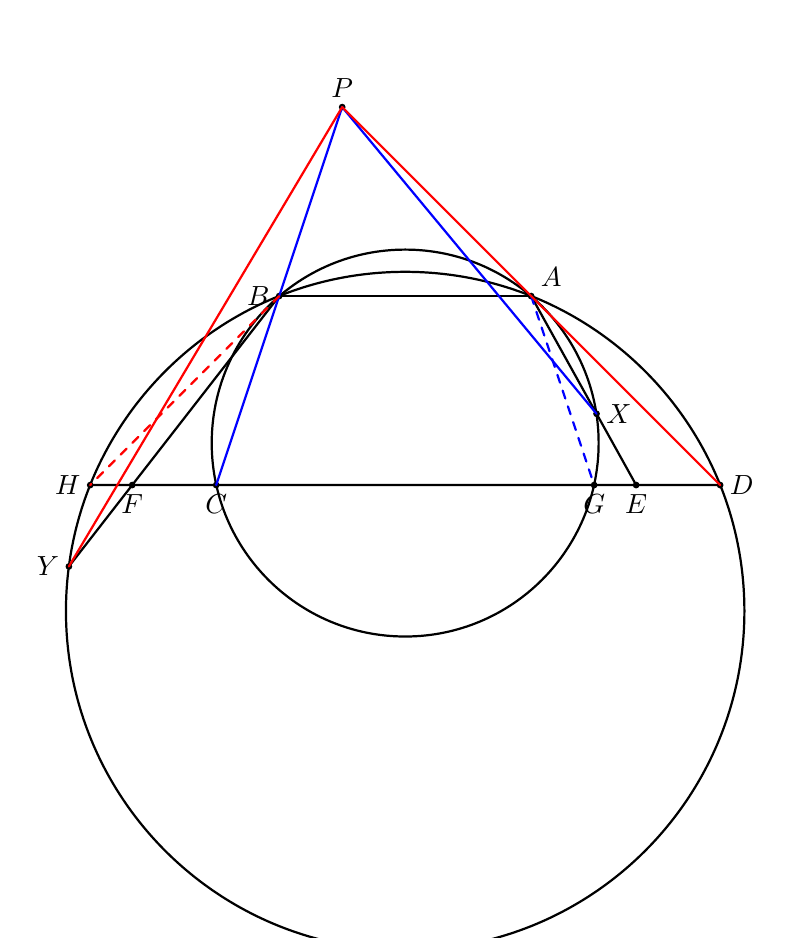
\begin{tikzpicture}[scale=0.8]
      % 1. 滿足 AB || CD 且 AB < CD，且非等腰
      \tkzDefPoint(2,3){A}
      \tkzDefPoint(-2,3){B}
      \tkzDefPoint(-3,0){C}
      \tkzDefPoint(5,0){D}
      
      % 2. 找到 AD 與 BC 的交點 P
      \tkzInterLL(A,D)(B,C) \tkzGetPoint{P}

      % 3. 找到三角形 ABC 和 ABD 的外心
      \tkzCircumCenter(A,B,C) \tkzGetPoint{O_1}
      \tkzCircumCenter(A,B,D) \tkzGetPoint{O_2}

      % 4. 找到C關於O_1P的對稱點X
      \tkzInterCC(O_1,C)(P,C) \tkzGetPoints{C_tmp}{X}
      % 5. 找到D關於O_2P的對稱點Y
      \tkzInterCC(O_2,D)(P,D) \tkzGetPoints{Y}{D_tmp}

      % 6. 繪製三角形 ABC 和 ABD 的外接圓
      \tkzDrawCircle[black,thick](O_1,A)
      \tkzDrawCircle[black,thick](O_2,A)

      % 7. 找到 AX 與 BY 的交點 Q
      %\tkzInterLL(A,X)(B,Y) \tkzGetPoint{Q}
      \tkzInterLL(A,X)(C,D) \tkzGetPoint{E}
      \tkzInterLL(B,Y)(C,D) \tkzGetPoint{F}
      \tkzInterLC(C,D)(O_1,A) \tkzGetPoints{C_tmp}{G}
      \tkzInterLC(C,D)(O_2,A) \tkzGetPoints{D_tmp}{H}

      \tkzDrawPoints[fill=black](A,B,C,D,E,F,X,G,H,Y,P)
      \tkzLabelPoints[below](C)
      \tkzLabelPoints[above right](A)
      %\tkzLabelPoints[above left](G)
      \tkzLabelPoints[left](B,H)
      \tkzLabelPoints[below](E,F,G)
      \tkzLabelPoints[above](P)
      %\tkzLabelPoints[above](Q)
      \tkzLabelPoints[right](X,D)
      \tkzLabelPoints[left](Y)
      \tkzDrawSegments[black, thick](A,B H,D A,E B,Y)
      \tkzDrawSegments[blue, thick](P,C P,X)
      \tkzDrawSegments[dashed, blue, thick](A,G)
      \tkzDrawSegments[dashed, red, thick](B,H)
      \tkzDrawSegments[red, thick](P,Y P,D)
    \end{tikzpicture}
  \end{center}
  第四步，「長度」轉換成「面積比值」：

  留意到$HC=GD$是已知事實，所以要證明命題四，等價於證明$HF$、$GE$分別在$HC$、$GD$內所佔的比值，即等價於以下的命題五：
  \begin{equation}
    HF=GE\Leftrightarrow \frac{HC}{HF}=\frac{GD}{GE}\Leftrightarrow\frac{HC}{HF}-1=\frac{GD}{GE}-1\Leftrightarrow\frac{FC}{HF}=\frac{ED}{GE}\label{eq:p2_s5}
  \end{equation}
  現在觀察$FC/HF$，常用的比值轉換手法就是「長度-面積」，即
  \begin{equation}
    \frac{FC}{HF}=\frac{\left[\triangle{CBY}\right]}{\left[\triangle{HBY}\right]}\label{eq:p2_s5-1}
  \end{equation}
  \begin{center}
      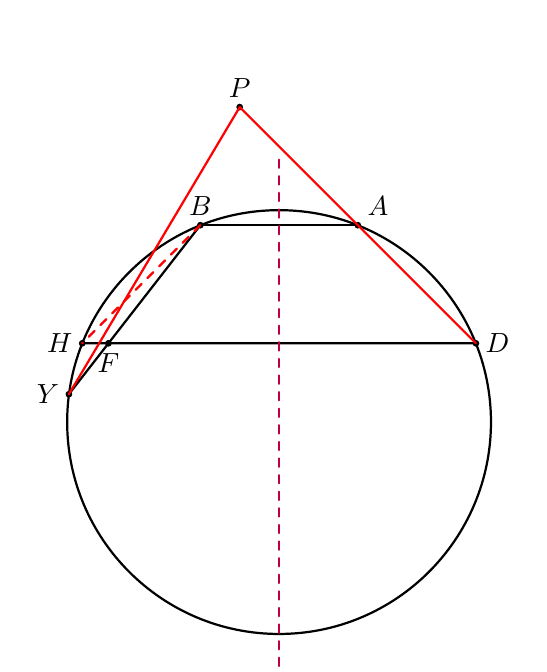
\begin{tikzpicture}[scale=0.5]
      % 1. 滿足 AB || CD 且 AB < CD，且非等腰
      \tkzDefPoint(2,3){A}
      \tkzDefPoint(-2,3){B}
      \tkzDefPoint(-3,0){C}
      \tkzDefPoint(5,0){D}
      
      % 2. 找到 AD 與 BC 的交點 P
      \tkzInterLL(A,D)(B,C) \tkzGetPoint{P}

      % 3. 找到三角形 ABC 和 ABD 的外心
      \tkzCircumCenter(A,B,C) \tkzGetPoint{O_1}
      \tkzCircumCenter(A,B,D) \tkzGetPoint{O_2}

      % 4. 找到C關於O_1P的對稱點X
      \tkzInterCC(O_1,C)(P,C) \tkzGetPoints{C_tmp}{X}
      % 5. 找到D關於O_2P的對稱點Y
      \tkzInterCC(O_2,D)(P,D) \tkzGetPoints{Y}{D_tmp}

      % 6. 繪製三角形 ABC 和 ABD 的外接圓
      %\tkzDrawCircle[black,thick](O_1,A)
      \tkzDrawCircle[black,thick](O_2,A)

      % 7. 找到 AX 與 BY 的交點 Q
      %\tkzInterLL(A,X)(B,Y) \tkzGetPoint{Q}
      \tkzInterLL(A,X)(C,D) \tkzGetPoint{E}
      \tkzInterLL(B,Y)(C,D) \tkzGetPoint{F}
      \tkzInterLC(C,D)(O_1,A) \tkzGetPoints{C_tmp}{G}
      \tkzInterLC(C,D)(O_2,A) \tkzGetPoints{D_tmp}{H}

      \tkzDrawPoints[fill=black](A,B,D,F,H,Y,P)
      %\tkzLabelPoints[below](C)
      \tkzLabelPoints[above right](A)
      %\tkzLabelPoints[above left](G)
      \tkzLabelPoints[left](H)
      \tkzLabelPoints[below](F)
      \tkzLabelPoints[above](P,B)
      %\tkzLabelPoints[above](Q)
      \tkzLabelPoints[right](D)
      \tkzLabelPoints[left](Y)
      \tkzDrawSegments[black, thick](A,B H,D B,Y)
      %\tkzDrawSegments[blue, thick](P,C P,X)
      %\tkzDrawSegments[dashed, blue, thick](A,G)
      \tkzDrawSegments[dashed, red, thick](B,H)
      \tkzDrawSegments[red, thick](P,Y P,D)
      \tkzDrawLine[purple, thick, dashed, add=1.5 and 2.5](O_1,O_2)
    \end{tikzpicture}
  \end{center}
  前面的部分有提及「線段$BA$和$HD$被同一條直線垂直平分」，所以有
  \begin{equation}
    \begin{aligned}
      \text{（中垂線）軸對稱：}&B\rightarrow A\\
      &H\rightarrow D
    \end{aligned}
    \quad\Rightarrow\quad BH=AD\label{eq:p2_s5-2}
  \end{equation}
  \begin{center}
      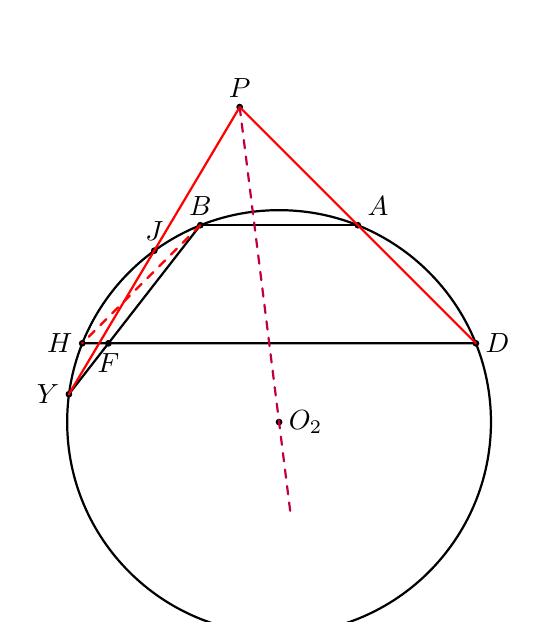
\begin{tikzpicture}[scale=0.5]
      % 1. 滿足 AB || CD 且 AB < CD，且非等腰
      \tkzDefPoint(2,3){A}
      \tkzDefPoint(-2,3){B}
      \tkzDefPoint(-3,0){C}
      \tkzDefPoint(5,0){D}
      
      % 2. 找到 AD 與 BC 的交點 P
      \tkzInterLL(A,D)(B,C) \tkzGetPoint{P}

      % 3. 找到三角形 ABC 和 ABD 的外心
      \tkzCircumCenter(A,B,C) \tkzGetPoint{O_1}
      \tkzCircumCenter(A,B,D) \tkzGetPoint{O_2}

      % 4. 找到C關於O_1P的對稱點X
      \tkzInterCC(O_1,C)(P,C) \tkzGetPoints{C_tmp}{X}
      % 5. 找到D關於O_2P的對稱點Y
      \tkzInterCC(O_2,D)(P,D) \tkzGetPoints{Y}{D_tmp}

      % 6. 繪製三角形 ABC 和 ABD 的外接圓
      %\tkzDrawCircle[black,thick](O_1,A)
      \tkzDrawCircle[black,thick](O_2,A)

      % 7. 找到 AX 與 BY 的交點 Q
      %\tkzInterLL(A,X)(B,Y) \tkzGetPoint{Q}
      \tkzInterLL(A,X)(C,D) \tkzGetPoint{E}
      \tkzInterLL(B,Y)(C,D) \tkzGetPoint{F}
      \tkzInterLC(C,D)(O_1,A) \tkzGetPoints{C_tmp}{G}
      \tkzInterLC(C,D)(O_2,A) \tkzGetPoints{D_tmp}{H}
      \tkzInterLC(P,Y)(O_2,A) \tkzGetPoints{J}{Y_tmp}

      \tkzDrawPoints[fill=black](A,B,D,F,H,Y,P,O_2,J)
      %\tkzLabelPoints[below](C)
      \tkzLabelPoints[above right](A)
      %\tkzLabelPoints[above left](G)
      \tkzLabelPoints[left](H)
      \tkzLabelPoints[below](F)
      \tkzLabelPoints[above](P,B,J)
      %\tkzLabelPoints[above](Q)
      \tkzLabelPoints[right](D,O_2)
      \tkzLabelPoints[left](Y)
      \tkzDrawSegments[black, thick](A,B H,D B,Y)
      %\tkzDrawSegments[blue, thick](P,C P,X)
      %\tkzDrawSegments[dashed, blue, thick](A,G)
      \tkzDrawSegments[dashed, red, thick](B,H)
      \tkzDrawSegments[red, thick](P,Y P,D)
      \tkzDrawLine[purple, thick, dashed, add=0 and 0.3](P,O_2)
    \end{tikzpicture}
  \end{center}  
  熟悉尺規作圖的讀者亦必然發現，$Y$點是$D$點關於「$P$點與$\triangle{ABD}$外心的連線」對稱的。作$\triangle{ABD}$外心為$O_2$，有
  \begin{align*}
    \text{（$PO_2$）軸對稱：}&A\rightarrow ??\\
    &D\rightarrow Y
  \end{align*}
  顯然「??」是$PY$與$\triangle{ABD}$外接圓且異於$Y$的另一個交點，記為$J$。由兩割線定理可知
  \begin{equation}
    PA=PJ,AD=JY\label{eq:p2_s5-2A}
  \end{equation}
  現時有結論如下：
  \begin{equation}
    BH=AD=JY\label{eq:p2_s5-3}
  \end{equation}
  由圓周角定理可知
  \begin{equation}
    \text{劣弧}HB=\text{劣弧}AD=\text{劣弧}YJ\quad\Rightarrow\quad\text{劣弧}YH=\text{劣弧}BJ\quad\Rightarrow\quad YH=BJ\label{eq:p2_s5-4}
  \end{equation}
  由(\ref{eq:p2_s5-3})和(\ref{eq:p2_s5-4})可知，$\triangle{HBY}\cong\triangle{JYB}$。所以(\ref{eq:p2_s5-1})式等價於
  \begin{equation}
    \frac{FC}{HF}=\frac{\left[\triangle{CBY}\right]}{\left[\triangle{JYB}\right]}\label{eq:p2_s5-5}
  \end{equation}
  同理，作$PX$與$\triangle{ABC}$外接圓且異於$X$的另一個交點，記為$I$，亦有
  \begin{equation}
    \frac{ED}{GE}=\frac{\left[\triangle{DAX}\right]}{\left[\triangle{IXA}\right]}\label{eq:p2_s5-6}
  \end{equation}
  所以要證明命題五等價於以下的命題六：
  \begin{equation}
    \frac{\left[\triangle{CBY}\right]}{\left[\triangle{JYB}\right]}=\frac{\left[\triangle{DAX}\right]}{\left[\triangle{IXA}\right]}\label{eq:p2_s6}
  \end{equation}
  整理當前幾何圖
  \begin{center}
      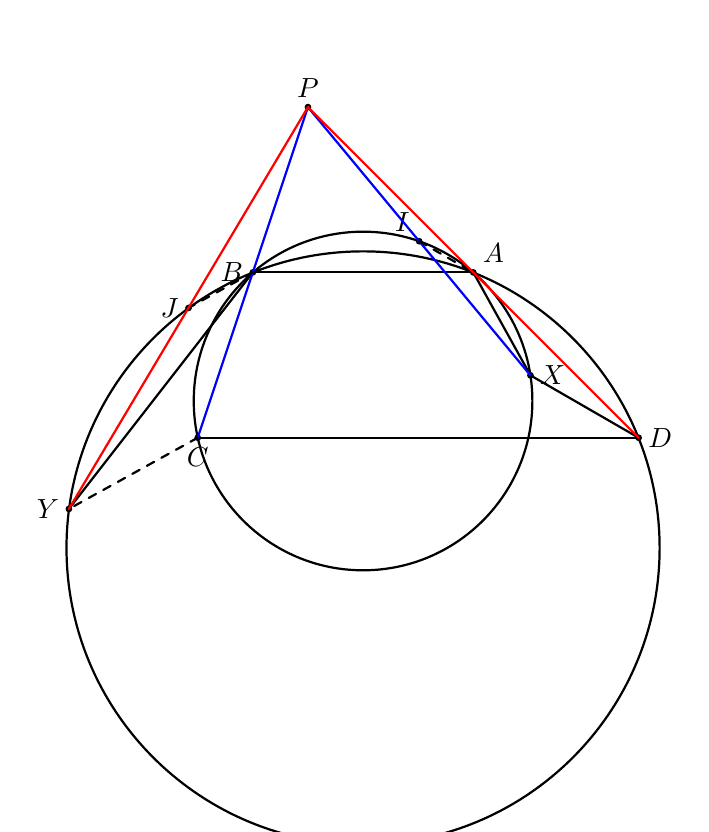
\begin{tikzpicture}[scale=0.7]
      % 1. 滿足 AB || CD 且 AB < CD，且非等腰
      \tkzDefPoint(2,3){A}
      \tkzDefPoint(-2,3){B}
      \tkzDefPoint(-3,0){C}
      \tkzDefPoint(5,0){D}
      
      % 2. 找到 AD 與 BC 的交點 P
      \tkzInterLL(A,D)(B,C) \tkzGetPoint{P}

      % 3. 找到三角形 ABC 和 ABD 的外心
      \tkzCircumCenter(A,B,C) \tkzGetPoint{O_1}
      \tkzCircumCenter(A,B,D) \tkzGetPoint{O_2}

      % 4. 找到C關於O_1P的對稱點X
      \tkzInterCC(O_1,C)(P,C) \tkzGetPoints{C_tmp}{X}
      % 5. 找到D關於O_2P的對稱點Y
      \tkzInterCC(O_2,D)(P,D) \tkzGetPoints{Y}{D_tmp}

      % 6. 繪製三角形 ABC 和 ABD 的外接圓
      \tkzDrawCircle[black,thick](O_1,A)
      \tkzDrawCircle[black,thick](O_2,A)

      % 7. 找到 AX 與 BY 的交點 Q
      %\tkzInterLL(A,X)(B,Y) \tkzGetPoint{Q}
      \tkzInterLL(A,X)(C,D) \tkzGetPoint{E}
      \tkzInterLL(B,Y)(C,D) \tkzGetPoint{F}
      \tkzInterLC(C,D)(O_1,A) \tkzGetPoints{C_tmp}{G}
      \tkzInterLC(C,D)(O_2,A) \tkzGetPoints{D_tmp}{H}
      \tkzInterLC(P,Y)(O_2,A) \tkzGetPoints{J}{Y_tmp}
      \tkzInterLC(P,X)(O_1,A) \tkzGetPoints{X_tmp}{I}

      \tkzDrawPoints[fill=black](A,B,C,D,X,Y,P,I,J)
      \tkzLabelPoints[below](C)
      \tkzLabelPoints[above right](A)
      \tkzLabelPoints[above left](I)
      %\tkzLabelPoints[above left](G)
      \tkzLabelPoints[left](B,J)
      %\tkzLabelPoints[below](E,F,G)
      \tkzLabelPoints[above](P)
      %\tkzLabelPoints[above](Q)
      \tkzLabelPoints[right](X,D)
      \tkzLabelPoints[left](Y)
      \tkzDrawSegments[black, thick](A,B X,D A,X B,Y C,D)
      \tkzDrawSegments[blue, thick](P,C P,X)
      \tkzDrawSegments[dashed, black, thick](B,J I,A C,Y)
      %\tkzDrawSegments[dashed, red, thick](B,H)
      \tkzDrawSegments[red, thick](P,Y P,D)
    \end{tikzpicture}
  \end{center}
  第六步，「面積比值」轉化成「長度比值」：
  \begin{align}
    \frac{\left[\triangle{CBY}\right]}{\left[\triangle{JYB}\right]}
    &=\frac{\left[\triangle{CBY}\right]/\left[\triangle{PBY}\right]}{\left[\triangle{JYB}\right]/\left[\triangle{PYB}\right]}\notag\\
    &=\frac{CB/BP}{JY/PY}\notag\\
    &=\frac{CB/BP}{AD/PD}\label{eq:p2_s6-1}
  \end{align}
  同理可得
  \begin{equation}
    \frac{\left[\triangle{DAX}\right]}{\left[\triangle{IXA}\right]}=\frac{DA/AP}{BC/PC}\label{eq:p2_s6-2}
  \end{equation}
  由「平行線分線段成比例」可知
  \begin{align}
    CB/BP&=DA/AP\\
    AD/PD&=BC/PC
  \end{align}
  由此可得
  \begin{equation}
    \frac{\left[\triangle{CBY}\right]}{\left[\triangle{JYB}\right]}=\frac{CB/BP}{AD/PD}=\frac{DA/AP}{BC/PC}=\frac{\left[\triangle{DAX}\right]}{\left[\triangle{IXA}\right]}\label{eq:p2_s6-3}
  \end{equation}
  命題六成立，即原命題得證。
\end{mybox}
\end{document}